%!TEX TS-program = xelatex
\documentclass[notes,12pt, aspectratio=169]{beamer}

\usepackage{amsmath,amsfonts,amssymb,amsthm,mathtools}  % пакеты для математики
%\usepackage{minted}

\usepackage[english, russian]{babel} % выбор языка для документа
\usepackage[utf8]{inputenc} % задание utf8 кодировки исходного tex файла
\usepackage[X2,T2A]{fontenc}        % кодировка

\usepackage{fontspec}         % пакет для подгрузки шрифтов
\setmainfont{Helvetica}  % задаёт основной шрифт документа

% why do we need \newfontfamily:
% http://tex.stackexchange.com/questions/91507/
\newfontfamily{\cyrillicfonttt}{Helvetica}
\newfontfamily{\cyrillicfont}{Helvetica}
\newfontfamily{\cyrillicfontsf}{Helvetica}

\usepackage{unicode-math}     % пакет для установки математического шрифта
% \setmathfont{Neo Euler} % шрифт для математики

\usepackage{polyglossia}      % Пакет, который позволяет подгружать русские буквы
\setdefaultlanguage{russian}  % Основной язык документа
\setotherlanguage{english}    % Второстепенный язык документа

% Шрифт для кода
\setmonofont[Scale=0.85]{Monaco}
\usepackage{verbments}

\usepackage{pgfpages}
% These slides also contain speaker notes. You can print just the slides,
% just the notes, or both, depending on the setting below. Comment out the want
% you want.
%\setbeameroption{hide notes} % Only slide
%\setbeameroption{show only notes} % Only notes
%\setbeameroption{show notes on second screen=right} % Both

\usepackage{array}

\usepackage{tikz}
\usepackage{verbatim}
\setbeamertemplate{note page}{\pagecolor{yellow!5}\insertnote}
\usetikzlibrary{positioning}
\usetikzlibrary{snakes}
\usetikzlibrary{calc}
\usetikzlibrary{arrows}
\usetikzlibrary{decorations.markings}
\usetikzlibrary{shapes.misc}
\usetikzlibrary{matrix,shapes,arrows,fit,tikzmark}

\usepackage{hyperref}
\usepackage{lipsum}
\usepackage{multimedia}
\usepackage{multirow}
\usepackage{dcolumn}
\usepackage{bbm}
\newcolumntype{d}[0]{D{.}{.}{5}}

\usepackage{changepage}
\usepackage{appendixnumberbeamer}
\newcommand{\beginbackup}{
   \newcounter{framenumbervorappendix}
   \setcounter{framenumbervorappendix}{\value{framenumber}}
   \setbeamertemplate{footline}
   {
     \leavevmode%
     \hline
     box{%
       \begin{beamercolorbox}[wd=\paperwidth,ht=2.25ex,dp=1ex,right]{footlinecolor}%
%         \insertframenumber  \hspace*{2ex} 
       \end{beamercolorbox}}%
     \vskip0pt%
   }
 }
\newcommand{\backupend}{
   \addtocounter{framenumbervorappendix}{-\value{framenumber}}
   \addtocounter{framenumber}{\value{framenumbervorappendix}} 
}

% для имитации питоновского синтаксиса 
\newcommand{\pgr}[1]{{\color{green} \textbf{#1}}}


%%%%%%%%%% Работа с картинками %%%%%%%%%
\usepackage{graphicx}                  % Для вставки рисунков
\usepackage{graphics}
\graphicspath{{images/}}    % можно указать папки с картинками
\usepackage{wrapfig}                   % Обтекание рисунков и таблиц текстом

\usepackage[space]{grffile}
\usepackage{booktabs}

% These are my colors -- there are many like them, but these ones are mine.
\definecolor{blue}{RGB}{0,114,178}
\definecolor{red}{RGB}{213,94,0}
\definecolor{yellow}{RGB}{240,228,66}
\definecolor{green}{RGB}{0,128, 0}

\hypersetup{
  colorlinks=false,
  linkbordercolor = {white},
  linkcolor = {blue}
}


%% I use a beige off white for my background
\definecolor{MyBackground}{RGB}{255,253,218}

%% Uncomment this if you want to change the background color to something else
%\setbeamercolor{background canvas}{bg=MyBackground}

%% Change the bg color to adjust your transition slide background color!
\newenvironment{transitionframe}{
  \setbeamercolor{background canvas}{bg=yellow}
  \begin{frame}}{
    \end{frame}
}

\setbeamercolor{frametitle}{fg=blue}
\setbeamercolor{title}{fg=black}
\setbeamertemplate{footline}[frame number]
\setbeamertemplate{navigation symbols}{} 
\setbeamertemplate{itemize items}{-}
\setbeamercolor{itemize item}{fg=blue}
\setbeamercolor{itemize subitem}{fg=blue}
\setbeamercolor{enumerate item}{fg=blue}
\setbeamercolor{enumerate subitem}{fg=blue}
\setbeamercolor{button}{bg=MyBackground,fg=blue,}


% If you like road maps, rather than having clutter at the top, have a roadmap show up at the end of each section 
% (and after your introduction)
% Uncomment this is if you want the roadmap!
% \AtBeginSection[]
% {
%    \begin{frame}
%        \frametitle{Roadmap of Talk}
%        \tableofcontents[currentsection]
%    \end{frame}
% }
\setbeamercolor{section in toc}{fg=blue}
\setbeamercolor{subsection in toc}{fg=red}
\setbeamersize{text margin left=1em,text margin right=1em} 

% списки, которые растягиваются на всю величину слайда 
\newenvironment{wideitemize}{\itemize\addtolength{\itemsep}{10pt}}{\enditemize}

\DeclareMathOperator{\Var}{Var}
\DeclareMathOperator{\E}{E}

\title[]{\textcolor{blue}{Глубокое обучение и вообще}}
\author{Ульянкин Филипп}
\date{ }

\usepackage[normalem]{ulem}

\begin{document}

%%% TIKZ STUFF
\tikzset{   
        every picture/.style={remember picture,baseline},
        every node/.style={anchor=base,align=center,outer sep=1.5pt},
        every path/.style={thick},
        }
\newcommand\marktopleft[1]{%
    \tikz[overlay,remember picture] 
        \node (marker-#1-a) at (-.3em,.3em) {};%
}
\newcommand\markbottomright[2]{%
    \tikz[overlay,remember picture] 
        \node (marker-#1-b) at (0em,0em) {};%
}
\tikzstyle{every picture}+=[remember picture] 
\tikzstyle{mybox} =[draw=black, very thick, rectangle, inner sep=10pt, inner ysep=20pt]
\tikzstyle{fancytitle} =[draw=black,fill=red, text=white]
%%%% END TIKZ STUFF

% Title Slide


\begin{frame}
\maketitle
\centering \textbf{\color{blue} Посиделка 6:}  Нейросети — конструктор LEGO (часть 1)
\end{frame}


\begin{frame}{Agenda}
\begin{wideitemize}
	\item  Какими бывают функции активации
	\item  Паралич  нейронной сети и взрыв градиентов 
	\item  Инициализация весов 
	\item  Переобучение нейронных сетей
	\item  Регуляризация: $l_1, l_2$, дропаут, ранняя остановка, их взаимосвязь
	\item  Первая порция советов по обучению нейросетей 	
\end{wideitemize} 
\end{frame}


\begin{transitionframe}
	\begin{center}
		\Huge Какими бывают функции активации
	\end{center}
	\centering \includegraphics[scale = 0.15]{act_f.png}
\end{transitionframe}


\begin{frame}{Сигмоида (sigmoid activation)}
\begin{center}
	\includegraphics[width=.9\linewidth]{sigmoid_activation_1.png}
\end{center}
\end{frame}


\begin{frame}{Сигмоида (sigmoid activation)}
\begin{center}
\includegraphics[width=.8\linewidth]{sigmoid_activation_2.png}
\end{center}
\end{frame}


\begin{frame}{Сигмоида (sigmoid activation)}
\begin{center}
	\includegraphics[width=.65\linewidth]{sigmoid_activation_2.png}
\end{center}

\begin{itemize}
	\item Сигмоида была популярна как классическая функция активации, но у неё есть ряд проблем
	{\color{red} 
	\item Насыщенные нейроны зануляют градиенты, в глубоких сетях возможен паралич
	}
\end{itemize}
\end{frame}


\begin{frame}{Затухание градиента (vanishing gradient problem)}
\begin{columns}
	\begin{column}{0.45\textwidth}
		\begin{wideitemize}
			\item  Изменение параметров в ходе обучения происходит на величину, которая  не влияет на выход сети
			
			\item Проблема связана с очень маленькими градиентами при обновлении весов:
			
			$$
			w_t = w_{t-1} - \gamma \cdot \nabla L(w_{t-1})
			$$
			
			\item При насыщении сети сигмоида убивает градиенты
		\end{wideitemize}
	\end{column}
	\hfill
	\begin{column}{0.55\textwidth}
		
		\begin{center}
			\only<1>{ 
				$$
				f(t) = \frac{1}{1 + e^{-t}}
				$$
				
				\includegraphics[width=0.98\textwidth]{sigm_der.png} 
			}
			
			% Сделать тут нормальную картинку 
			\only<2>{
				\includegraphics[width=0.98\textwidth]{vanishing_loss.png} 
				
				\mbox{  }
				
				\alert{Толи обучение сошлось, толи веса просто больше не обновляются \ldots}
			}
		\end{center} 
	\end{column}
\end{columns}
\end{frame}


\begin{frame}{Паралич сети}
	\begin{wideitemize}
		\item  В случае сигмоиды $\sigma'(x) = \sigma(x) \cdot (1 - \sigma(x))$ 
		
		\item Сигмоида принимает значения на отрезке $[0; 1]$, значит максимальное значение её производной это $^1/_4$
		
		\item Если сеть очень глубокая, происходит \alert{затухание градиента} 
		
		\item Градиент затухает экспоненциально $\Rightarrow$ сходимость замедляется, более ранние веса обновляются дольше, более глубокие веса быстрее  $\Rightarrow$ значение градиента становится ещё меньше $\Rightarrow$ наступает \alert{паралич сети} 
		
		\item В сетях с небольшим числом слоёв этот эффект незаметен
	\end{wideitemize} 
\end{frame}


\begin{frame}{Взрыв градиента (exploding gradient problem)}
\begin{columns}
	\begin{column}{0.4\textwidth}
		\begin{wideitemize}
			\item  Изменение параметров в ходе обучения происходит на очень большую величину и обучение деградирует
			
			\item Проблема связана с очень большими градиентами при обновлении весов:
			
			$$
			w_t = w_{t-1} - \gamma \cdot \nabla L(w_{t-1})
			$$
			
		\end{wideitemize}
	\end{column}
	\hfill
	\begin{column}{0.6\textwidth}
		
		\begin{center}
				\includegraphics[width=0.98\textwidth]{exp_grad.png} 
		\end{center} 
	\end{column}
\end{columns}
\end{frame}


\begin{frame}{Взрыв и затухание градиента}
	\begin{wideitemize}
		\item Затухание градиента связано не только с сигмоидой
		\item Взрыв градиента также встречается довольно часто 
		\item $\Rightarrow$ грамотные инициализация и оптимизация
		\item $\Rightarrow$ разработка новых архитектур и специальных слоёв
	\end{wideitemize}
\end{frame}


\begin{frame}{Сигмоида (sigmoid activation)}
\begin{center}
	\includegraphics[width=.65\linewidth]{sigmoid_activation_2.png}
\end{center}

\begin{itemize}
	{\color{red} 
		\item Насыщенные нейроны зануляют градиенты, в глубоких сетях возможен паралич
		\item Не центрирована относительно нуля
	}
		\item Что мы можем сказать о градиентах нейрона с сигмоидой? 
\end{itemize}
\end{frame}


\begin{frame}{Центрирование относительно нуля}
\begin{columns}
	\begin{column}{0.6\textwidth}
		\begin{wideitemize}
			\item  Выход слоя мы обычно находим как 
			
			\[
			o_i = \sigma(h_i)
			\]
			
			\item он всегда положительный, значит градиент по весам, идущим на вход в текущий нейрон тоже положительные 
			\item $\Rightarrow$ все веса обновляются в одинаковом направлении 
			\item $\Rightarrow$ сходимость идёт медленнее, причём зиг-загами
		\end{wideitemize} 
	\end{column}
	\hfill
	\begin{column}{0.4\textwidth}
		
		\begin{center}
			\includegraphics[width=0.98\textwidth]{gr_update.png} 
		\end{center} 
	\end{column}
\end{columns}
\end{frame}



\begin{frame}{Сигмоида (sigmoid activation)}
\begin{center}
	\includegraphics[width=.65\linewidth]{sigmoid_activation_2.png}
\end{center}

\begin{itemize}
	{\color{red} 
		\item Насыщенные нейроны зануляют градиенты, в глубоких сетях возможен паралич
		\item Не центрирована относительно нуля
		\item Вычислять $e^x$ дорого
	}
\end{itemize}
\end{frame}


\begin{frame}{Гиперболический тангенс (tanh activation)}
	\begin{center}
		\includegraphics[width=.8\linewidth]{tanh_activation.png}
	\end{center}
	\begin{itemize}
		\item  {\color{green}  Центрирован относительно нуля }
		
		\item  {\color{red}  Всё ещё похож на сигмоиду }
		
		\item $f'(x) = 1 - f(x)^2$  $\Rightarrow$ затухание градиента
	\end{itemize}
\end{frame}


\begin{frame}{Rectifier Linear Unit activation, ReLU (2012)}
	\begin{center}
		\includegraphics[width=.8\linewidth]{relu_activation.png}
	\end{center}
	\begin{itemize}
		{ \color{green} 
		\item  Быстро вычисляется 
		\item  Градиенты не угасают при $x > 0$
		\item  На практике ускоряет сходимость
		} 
	\end{itemize}
\end{frame}


\begin{frame}{ReLU (2012)}
	\begin{center}
		\includegraphics[width=.8\linewidth]{relu_activation.png}
	\end{center}
	\begin{itemize}
		{ \color{red} 
		\item  Сетка может умереть, если активация занулится на всех нейронах
		\item  Не центрирован относительно нуля
		} 
	\end{itemize}
\end{frame}


\begin{frame}{Зануление ReLU}
	\begin{center}
		\includegraphics[width=.8\linewidth]{relu_activation.png}
	\end{center}
	\begin{wideitemize}
		\item   $f(x) = \max(0, w_0 + w_1 \cdot h_1 + \ldots + w_k \cdot h_k)$
		
		\item  Если $w_0$ инициализировано большим отрицательным числом, нейрон сразу умирает $\Rightarrow$ надо аккуратно инициализировать веса
	\end{wideitemize}
\end{frame}


\begin{frame}{Leaky ReLU activation (2013)}
\begin{center}
\includegraphics[width=.8\linewidth]{leaky_relu_activation.png}
\end{center}

\begin{itemize}
{ \color{green} 
\item Как ReLU, но не умирает, всё ещё легко считается
\item Производная может быть любого знака
\item Важно, чтобы $a \ne 1$, иначе линейность} 
{\color{red} 
\item  Не центрирован относительно нуля} 
\end{itemize}
\end{frame}


\begin{frame}{Exponential Linear Units activation, ELU (2015)}
	\begin{center}
		\includegraphics[width=.8\linewidth]{elu.png}
	\end{center}
	\begin{columns}
		\begin{column}{0.7\textwidth}
			\begin{itemize}
				{ \color{green} 
					\item  Примерно центрирован в нуле (в контексте математического ожидания)
					\item  Сходимость быстрее ReLU
					\item  На практике ускоряет сходимость} 
			\end{itemize}
		\end{column}
		\hfill
		\begin{column}{0.4\textwidth}
			\includegraphics[width=.55\linewidth]{elu_loss.png}
		\end{column}
	\end{columns}
\vfill %
\footnotesize
{\color{blue} \url{https://arxiv.org/pdf/1511.07289.pdf}}
\end{frame}


\begin{frame}{Scaled Exponential Linear Units activation, SELU (2017)}
\begin{columns}
	\begin{column}{0.45\textwidth}
		\begin{center}
			\includegraphics[width=.99\linewidth]{selu.png}
		\end{center}
	\end{column}
	\hfill
	\begin{column}{0.55\textwidth}
		\begin{wideitemize} 
				\item  Нормализованная версия ELU, лучше работает для глубоких сетей
				\item  Обладает свойством самонормализации
				\item  Можно учить сетки без нормализации по батчам (будем обсуждать позже)
		\end{wideitemize}
	\end{column}
\end{columns}
\vfill %
\footnotesize
{\color{blue} \url{https://arxiv.org/abs/1706.02515}}
\end{frame}

\begin{frame}{Swish (2017)}
	\begin{columns}
		\begin{column}{0.35\textwidth}
			\begin{center}
				\includegraphics[width=.95\linewidth]{swish.png}
				\[f(x) = x \cdot \sigma(\beta x) \]
			\end{center}
		\mbox{    } параметр $\beta$ обучается
		\end{column}
		\hfill
		\begin{column}{0.65\textwidth}
			\begin{itemize} 
				\item  В 2017 году Google Brain хитрым автоматическим поиском на основе RNN нашла функцию активации Swish, работающую лучше ReLU
			\end{itemize}
		\begin{center}
			\includegraphics[width=.99\linewidth]{swish_can.png}
		\end{center}
		\end{column}
	\end{columns}
\vfill %
\footnotesize
{\color{blue} \url{https://arxiv.org/abs/1710.05941} \newline \url{https://krutikabapat.github.io/Swish-Vs-Mish-Latest-Activation-Functions/} }
\end{frame}


\begin{frame}{Mish (2019)}
	\begin{columns}
		\begin{column}{0.5\textwidth}
			\begin{center}
				\includegraphics[width=.9\linewidth]{mish.png}
			\end{center}
		\end{column}
		\hfill
		\begin{column}{0.5\textwidth}
			Похожим образом получили функции активации Mish
				\[f(x) = x \cdot tanh(\ln(1 + e^x)) \]
		\end{column}
	\end{columns}
	\vfill %
	\footnotesize
	{\color{blue} \url{https://arxiv.org/pdf/1908.08681.pdf} \newline \url{https://krutikabapat.github.io/Swish-Vs-Mish-Latest-Activation-Functions/} }
\end{frame}


\begin{frame}{Activate or Not, ACON (2020)}
\begin{wideitemize} 
	\item  Swish -- гладкий вариант ReLU с гейтом 
	\item  Функция сама решает, нужна слою активация или нет 
	\item  Можно обобщить этот подход и придумать более интересные функции потерь, которые дадут улучшение
\end{wideitemize}	
\vfill %
\footnotesize
{\color{blue} \url{https://arxiv.org/pdf/2009.04759.pdf}}
\end{frame}


%Подход в общем классический. Давайте поймём как имеющиеся функции можно обобщить, а потом из этого обобщения предложим что-нибудь интересное. Заодно и интуицию обретём.
%
%Логические шаги тут следующие:

%1. Функцию max можно аппроксимировать гладким и дифференцируемым вариантом, который мы будем называть smooth maximum с параметром β, который когда стремится к бесконечности, даёт в пределе максимум, а когда стремится к нулю — арифметическое среднее.
%
%S_β(x_1, ..., x_n) = sum(x_i*exp(β*x_i))/sum(exp(β*x_i))
%
%2. ReLU это, как известно, max(x,0), а значит можно аппроксимировать этим нашим гладким максимумом о двух входах: 
%
%S_β(η_a(x), η_b(x))
%и η_a(x) = x, η_b(x) = 0,
%
%3. Swish тоже можно представить через эту функцию S_β(x, 0) = x * σ(β*x) и её мы называем ACON-A. А заодно Swish — это гладкая аппроксимация ReLU.
%
%4. Если рассмотреть развития ReLU типа PReLU, Leaky ReLU и т.п., то можно прийти к функции ACON-B c n η_a(x) = x, η_b(x) = px.
%
%5. Можно пойти ещё дальше и сделать ACON-C с η_a(x) = p_1*x, η_b(x) = p_2*x(p_1 != p_2). ACON-C в такой формулировке позволяет иметь обучаемые верхние и нижние границы для градиента (у Swish они фиксированы). Они определяются параметрами p_1 и p_2.
%
%6. Ну и наконец параметр β тоже можно обучать и это даёт функцию Meta-ACON. Этот параметр называется switching factor и регулирует поведение нейрона: линейный (неактивный нейрон) или нелинейный режим работы (активный нейрон). Отсюда и название ActivateOrNot (ACON).
%
%И вот эта последняя история открывает целое пространство для исследования, можно реализовывать разные функции, генерящие эту β по входным данным: можно иметь общий параметр на весь слой, можно на отдельные каналы, а можно и на пиксели.
%
%Что вообще даёт вся эта эквилибристика? На редкость неплохие улучшения, единицы процентных пунктов в терминах top-1 ошибки. Для которых от вас по большому счёту ничего не требуется кроме замены функции активации.
%
%Ну и заодно вроде понятнее стало, что такое Swish и вообще.


\begin{frame}{ TLDR: что на практике}
	\begin{wideitemize}
		\item Начните с ReLU, аккуратно инициализируйте веса и настраивайте скорость обучения
		\item Попробуйте Leaky ReLU / ELU / SELU / Swish / Mish, если есть время на эксперименты, чтобы выжать максимум
		\item Не используйте сигмоиду и  tanh
	\end{wideitemize}
\vfill %
\footnotesize
Краткий обзор функций активаций: {\color{blue}  \url{https://arxiv.org/pdf/1804.02763.pdf}}
\end{frame}


\begin{transitionframe}
	\begin{center}
		\Huge  Предобработка данных
	\end{center}
\centering 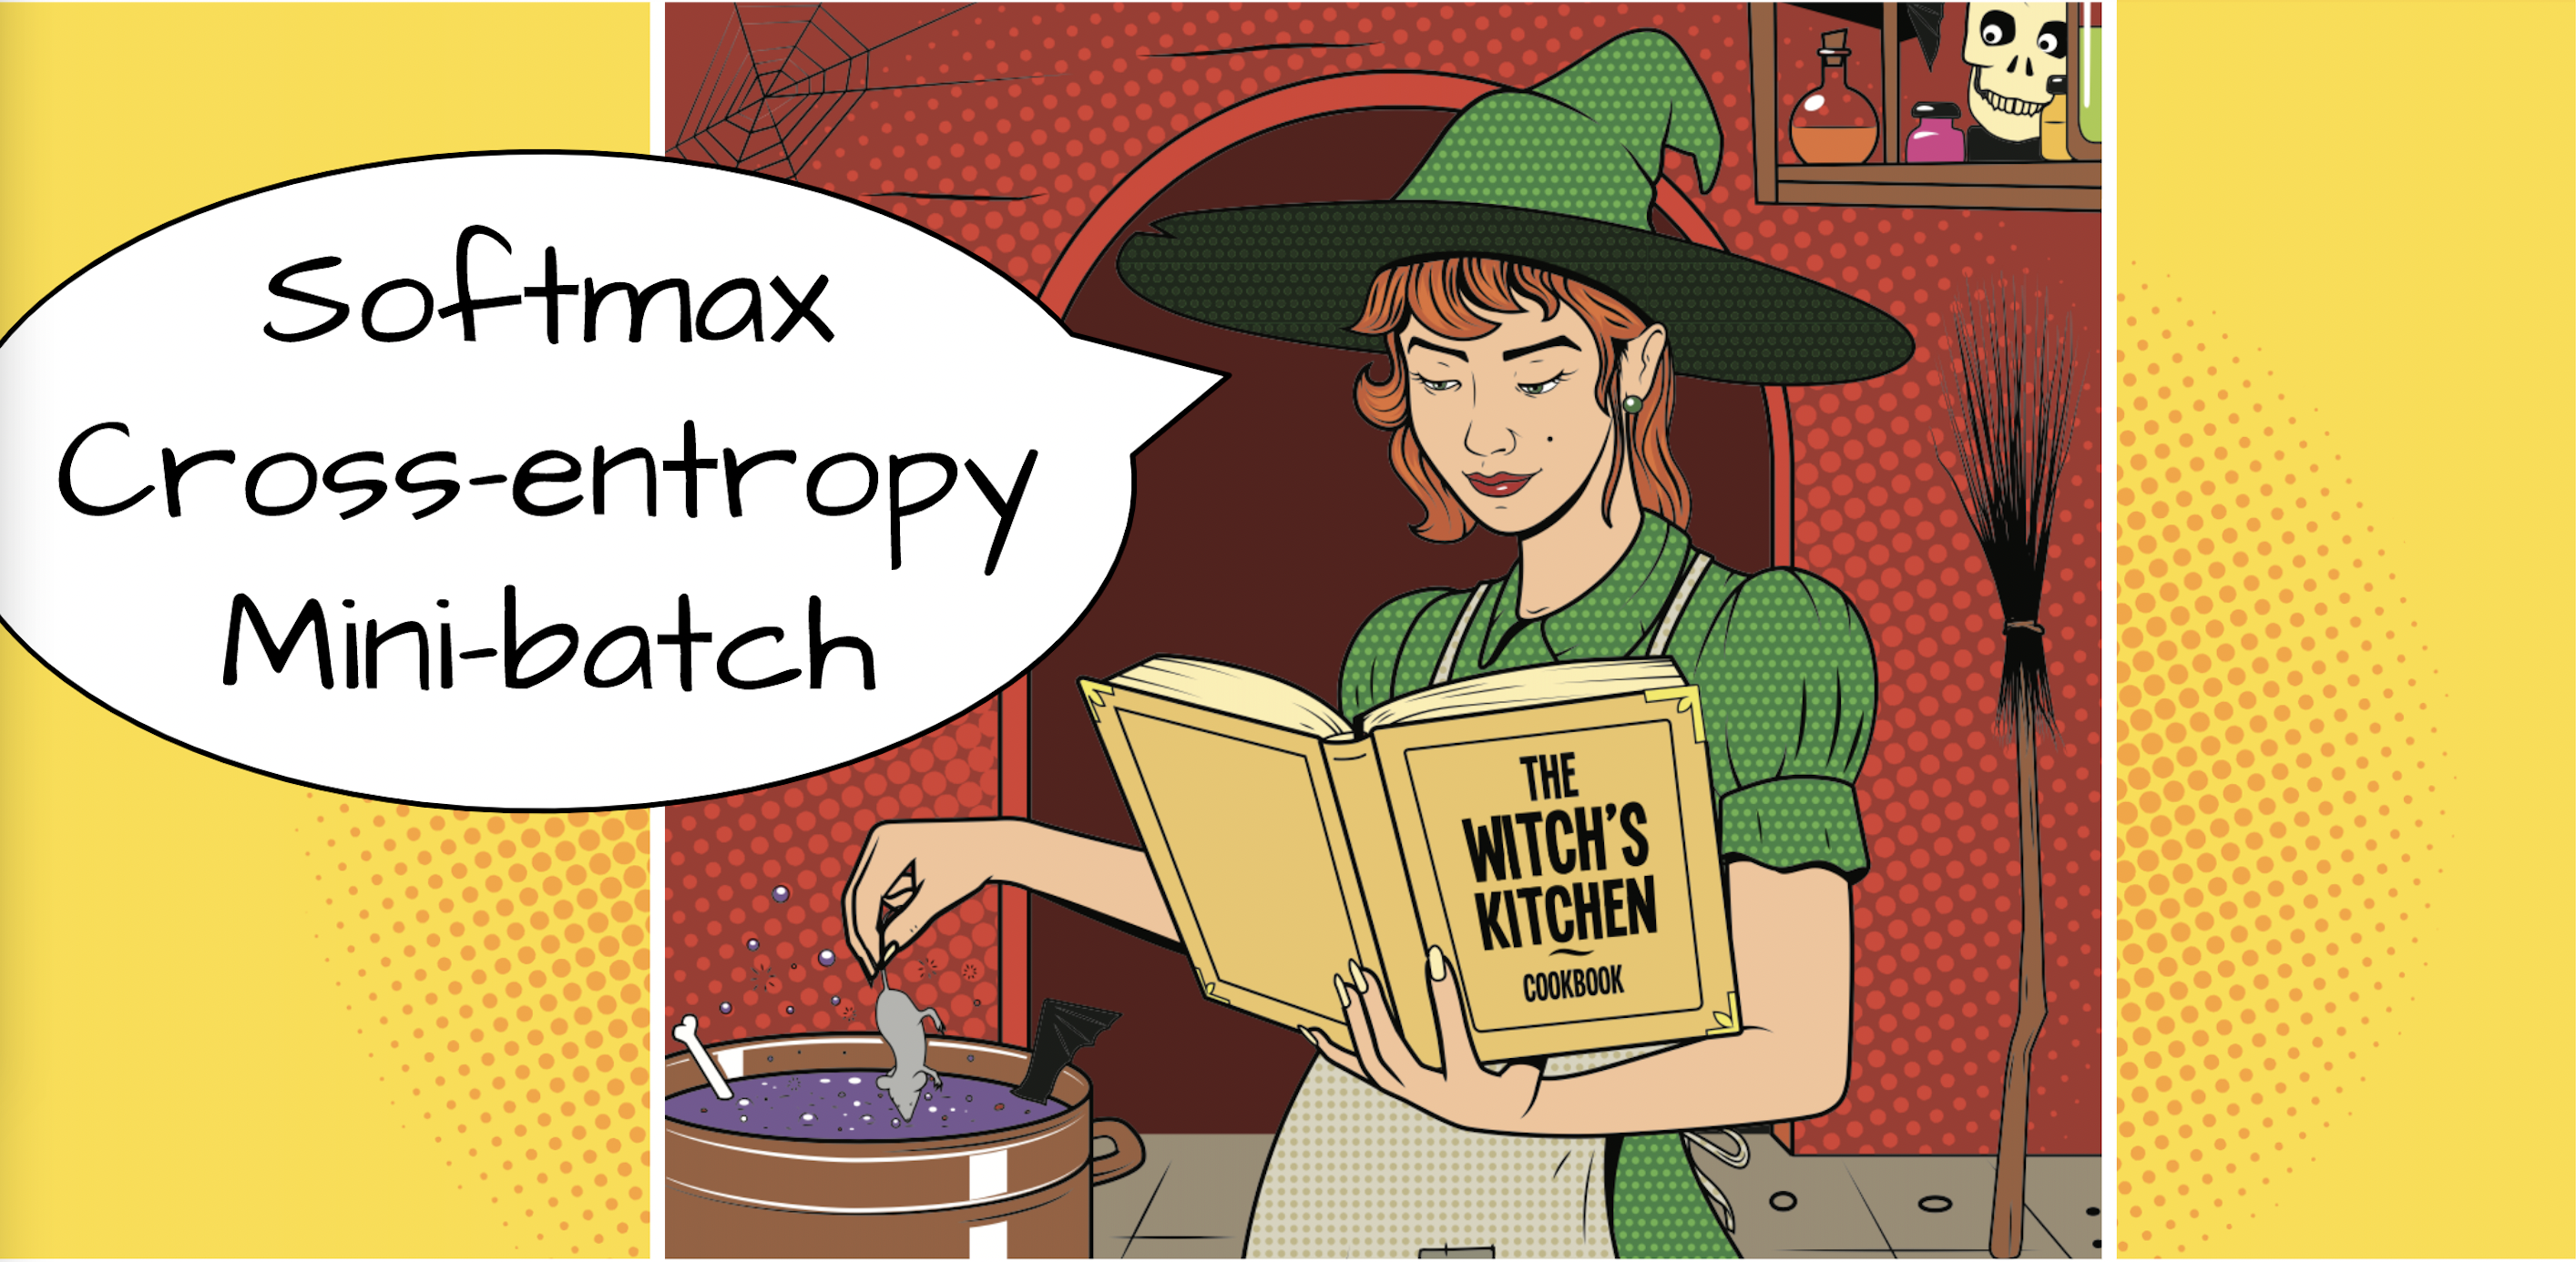
\includegraphics[scale = 0.2]{prepare.png}
\end{transitionframe}


\begin{frame}{Предобработка данных}
\begin{center}
	\includegraphics[width=0.99\paperwidth]{data_norm.png}
\end{center}
\vfill %
\footnotesize
{\color{blue}  \url{http://cs231n.stanford.edu/slides/2021/}}
\end{frame}


\begin{frame}{Предобработка табличных данных}
	\begin{columns}
	\begin{column}{0.5\textwidth}
		\alert{Без нормализации}
		\includegraphics[width=.95\linewidth]{no_prep.png}
	\end{column}
	\hfill
	\begin{column}{0.5\textwidth}
		\alert{С нормализацией}
		\includegraphics[width=.95\linewidth]{with_prep.png}
	\end{column}
\end{columns}
\end{frame}


\begin{frame}{Зачем нормализация картинкам?}
\begin{columns}
	\begin{column}{0.6\textwidth}
			\begin{wideitemize}
			\item \alert{Что происходит, когда все входы в нейрон положительные?}
			\item Все градиенты либо положительные либо отрицательные 
			\item Картинки центрируют для того, чтобы были отрицательные входы
			\item Картинки нормируют, чтобы инициализированным в окрестности нуля весам легче было сходиться
		\end{wideitemize}
	\end{column}
	\hfill
	\begin{column}{0.4\textwidth}
		
		\begin{center}
			\includegraphics[width=0.98\textwidth]{gr_update.png} 
		\end{center} 
	\end{column}
\end{columns}
\end{frame}


\end{document}